\documentclass[12pt]{scrreprt}
\usepackage[utf8]{inputenc}
\usepackage[ngerman]{babel}
\usepackage[utf8]{inputenc}
\usepackage[T1]{fontenc}
\usepackage{hyperref}

%\hypersetup{colorlinks=true, citecolor=red}


\usepackage{natbib}
\usepackage[numbib]{tocbibind}
\usepackage{float}
\linespread{1.3}
\usepackage{natbib}
\usepackage{graphicx}
\usepackage{pdfpages}
\usepackage[euler]{textgreek}
\usepackage{adjustbox}
\usepackage[margin = 3cm]{geometry}


\usepackage{eso-pic} 
\usepackage{lipsum} 

\usepackage{tabularx} 
\usepackage{multirow}
\usepackage{amssymb}
\usepackage[flushleft]{threeparttable}
\usepackage{booktabs,caption}

\usepackage{amsmath}
\usepackage{bbm}
\usepackage{bbold}





\pagenumbering{roman}

\begin{document}
	
	\pagestyle{myheadings}

\chapter{Methodik}
In diesem Kapitel wird als erstes die Theorie hinter den Modellen erklärt. Danach gehen wir auf die Schwierigkeiten ein, denen wir gegenüberstanden. Im letzten Teil stellen wir, dann die Ergebnisse vor.
\section{Theorie}
In folgendem Kapitel soll in einem Modell der Zusammenhang einer beobachteten abhängigen Variable, in unserem Fall, der Anteil der Skitourengänger mit LVS-Gerät, durch mehrere unabhängige Variablen erklärt werden.
Für das bessere Verständis bauen wir den Theorie-Teil von einem einfachen Modell bis hin zu dem von uns verwendeten Modell auf.
\subsection{Lineares Regressionsmodell}
Bei einem linearen Regressionsmodell wird der Erwartungswert einer Zielvariable durch die Linearkombination von Einflussgrö"sen, auch Kovariablen genannt, beschrieben. Das lineare Regressionsmodell nimmt dabei folgende Form an:
\begin{align}
y_{i}= \beta_{0}+\beta_{1}x_{i1}+...+\beta_{k}x_{ik}+\epsilon_{i}
\end{align}
Die Zielgrö"se wird durch $y_{i}$ abgebildet, welche im Fall des linearen Regressionsmodells normalverteilt ist. Die Kovariablen werden durch $x_{i1},...,x_{ik}$ gekennzeichnet und $\epsilon_{i}$ stellt den Störterm dar. In Anwendungen bei denen es sich nicht um eine normalverteilte Zielvariable handelt ist das lineare Regressionsmodell unzureichend. Um das Problem zu lösen, wird im nächsten Kapitel auf das generalisierte lineare Regressionsmodell eingegangen. (Quelle: Fahrmeir S.62)
\subsection{Generalisierte lineare Regressionsmodell}
Das generalisierte lineare Regressionsmodell eignet sich für die Modellierung von Zielvariablen die nicht unbedingt normalverteilt sind. Die abhängige Variable nimmt typischerweise eine Verteilung aus einer Exponentialfamilie (z.B. Binomial, Poisson, Multinomial, Normal,...) an. In unserem Fall handelt es sich um eine durch 0 und 1 kodierte Zielvariable $y_{i}$. Die beobachtete Zielgrö"se, der Anteil an Personen mit LVS-Gerät, ist Binomial-verteilt mit $y_{i}|x_{i}\sim B(1,\pi_{i})$: \\
\begin{align}
%\vspace{0.1cm}
y_{i}=\begin{cases}
1 & \text{,wenn Person mit LVS-Gerät identifiziert wird } \\
0 & \text{,wenn Person ohne LVS-Gerät identifiziert wird.} \\
\end{cases}
\end{align}
Bei der generalisierten Regression mit binärer Zielvariable wird der Effekt der Kovariablen durch die (bedingte) Wahrscheinlichkeit $\pi_{i}$ beschrieben.
\begin{align}
\pi_{i}=P(y_{i}=1|x_{i1},...,x_{ik})=E(y_{i}|x_{i1},...,x_{ik})
\end{align}
Für den Erwartungswert der Zielvariable gilt:
\begin{align}
E(y_{i})=\pi_{i}=\frac{exp(\eta_{i})}{1+exp(\eta_{i})}=h(\eta_{i}).
\end{align}
Der Erwartungswert der Zielvariable wird mit dem linearen Prädiktor $\eta_{i}$ mittels der Responsefunktion $\pi_{i}=h(\eta_{i})$ verknüpft. Die Logit-Linkfunktion $g$ ist die Umkehrung der Responsefunktion, daher gilt:
\begin{align}
g(\pi_{i})=\log(\frac{\pi_{i}}{1-\pi_{i}}).
\end{align}
In unserer Arbeit machen wir Gebrauch von dem Logit-Link. Diese Transformation ist zur mathematischen Berechnung unseres Modells notwendig. In Kapitel (...) werden wir den Logit-Link zurücktransformieren um die Interpretation der Ergebnisse zu vereinfachen.
Das generalisierte lineare Regressionsmodell beschreibt lineare Einflüsse der Kovariablen auf die Zielvariable. In praktischen Anwendungen ist dies oft unzureichend, da neben den linearen Einflüssen auch nicht-lineare, flexible Einflüsse von Kovariablen auf die abhängige Variable wirken können (Quelle: Fahrmeir S.190). Daher wird im nächsten Kapitel die additive Regression näher erläutert.
\subsection{Additives Regressionsmodell}
Das additive Modell stellt in der Statistik ein semi-parametrisches Regressionsmodell dar. Neben mehreren nicht-linearen flexiblen Einflüssen können hier auch lineare Einflüsse von Kovariablen auf die abhängige Variable modelliert werden. \\
Das Standardmodell der additiven Regression hat die Form:
\begin{align}
y_{i}=\underbrace{\beta_{0}+\beta_{1}x_{i1}+...+\beta_{k}x_{ik}}_{\text{parametrische Effekte}}+ \underbrace{f_{1}(z_{i1})+...+f_{q}(z_{iq})}_{\text{semi-parametrische Effekte}}+\epsilon_{i}
\end{align}
Der parametrische Teil des Standardmodells hat die gleiche Form, wie schon im linearen Modell aufgezeigt. Die Funktionen $f_{1}(z_{1}),...,f_{q}(z_{q})$ werden mit nichtparametrischen Effekten geschätzt. (Quelle: Fahrmeir S.47)
Auf die Theorie hinter der Funktion $f$ wird im nächsten Kapitel eingegangen.
\subsection{Splines}
Die Schätzfunktion $f$ wird durch sogenannte Splines modelliert. Splines stellen bestimmte Funktionen dar, die stückweise aus Polynomen eines bestimmten Grades zusammengesetzt werden. Es gibt verschiedene Arten von Splines. In unserer Arbeit beschränken wir uns auf die Penalisierten Splines, die Zyklische Splines und die Thin-Plate Splines.
\subsubsection{Polynom-Splines}
	Eine Möglichkeit, die Funktion $f$ abzubilden, sind Splines, die über Polynome modelliert werden und Polynom-Splines, oder auch Regressions-Splines, genannt werden. Das polynomiale Modell hat die Form: 
\begin{align}
f(z)=\gamma_{0}+\gamma_{1}z+...+\gamma_{l}z^l,
\end{align}
wobei das Polynom vom Grad $l$ durch den Einfluss von $z$ auf $y$ modelliert wird und $\gamma_{j}$ die Regressionskoeffizienten darstellen. Um eine flexible Schätzfunktion gewährleisten zu können, wird der Definitionsbereich von $z$ in Intervalle geteilt und Polynome werden für das jeweilige Intervall geschätzt. Die Zerlegung von $z$ erfolgt stückweise auf Basis von sogenannten Knotenmengen $k_{1}$ bis $k_{m}$.  Ein Problem, welches dabei entstehen könnte ist, dass an den Intervallgrenzen keine $glatte$ Funktion entstehen. Der Graph einer $glatten$ Funktion hat an den Intervallgrenzen keine \glqq{Ecken\grqq}. Deshalb muss für die \glqq{mathematische}\grqq ~Glattheit die zusätzliche Bedingung, dass die Funktion $f(z)$ an den Intervallgrenzen $(l-1)$-mal stetig differenzierbar ist, eingeführt werden. Der Grad des Splines und die Anzahl der Knoten können somit im hohen Ma"se die Funktion beeinflussen, je höher die Anzahl an Knoten ist, desto $rauer$ ist die Funktion $f(z)$. Um Polynom-Splines in der Praxis anwenden zu können, bedarf es einer Darstellung der Menge der Polynom-Splines. Eine mögliche Darstellung eines Polynom-Splines stellt die B-Spline-Basisfunktion dar.
\subsubsection{Basis Splines}
Der B-Spline dient als Basisfunktion für Polynom-Splines. Jedoch wird sich auch der Penalisierungs-Spline, welcher im darauffolgenen Kapitel vorgestellt wird, die B-Spline-Basisfunktion zu Nutzen machen. Das Ziel bei der Konstruktion der B-Spline-Basisfunktion ist es die Polynomstücke des gewünschten Grades an den Knoten ausreichend $glatt$ zusammenzusetzen. Die Basisfunktion besteht dabei aus $(l+1)$ Polynomstücken vom Grad $l$, welche stetig an den Knoten zusammengesetzt werden. Die Funktion $f(z)$ lässt sich durch die Linearkombination der Basisfunktionen:
\begin{align}
f(z)=\sum_{j=1}^d\gamma_{j}B_{j}(z)
\end{align}
darstellen. Die Koeffizienten  $\gamma_{j}$ werden mit Hilfe der KQ-Methode geschätzt und dienen zur Skalierung der Basisfunktionen. Die Anzahl der erforderlichen Basisfunktionen $d = m+l-1$, setzt sich aus der Zahl der Knoten $m$ und den Polynomstücken des gewünschten Grades $l$, welche $(l-1)$-mal stetig differenzierbar an den Knoten aneinandergefügt werden, zusammen.  \\
Für B-Splines vom Grad 0 folgt:
\begin{align}
B_{j}^0(z)= \mathbb{1}_{[k_{j},k_{j+1}]}(z)= 
\begin{cases}
1 & k_{j} \leq z<k_{j+1};\enspace mit\enspace j=1,...,d-1; \\
0 & \text{sonst.} \\
\end{cases}
\end{align}
Für B-Splines höheren Grades gilt:
\begin{align}
B_{j}^l(z)= \frac{z-k_{j}}{k_{j+l}-k_{j}}B_{j}^{l-1}(z)+
\frac{k_{j+l+1}-z}{k_{j+l+1}-k_j+1}B_{j+1}^{l-1}(z).
\end{align}
Die Abbildung \ref{pic:b_spline} visualisiert die Schätzung eines B-Splines anhand eines fiktiven Datenbeispiels schematisch. Abbildung (a) demonstriert eine B-Spline Basis vom dritten Grad. In Abbildung (b) wird die Basisfunktion mit dem Kleinste-Quadrate-Schätzer $\hat\gamma_{j}$ skaliert. Die Abbildung (c), zeigt die erhaltene Schätzung, wenn die skalierten Basisfunktionen addiert werden.
\begin{figure}[H]
	\centering
	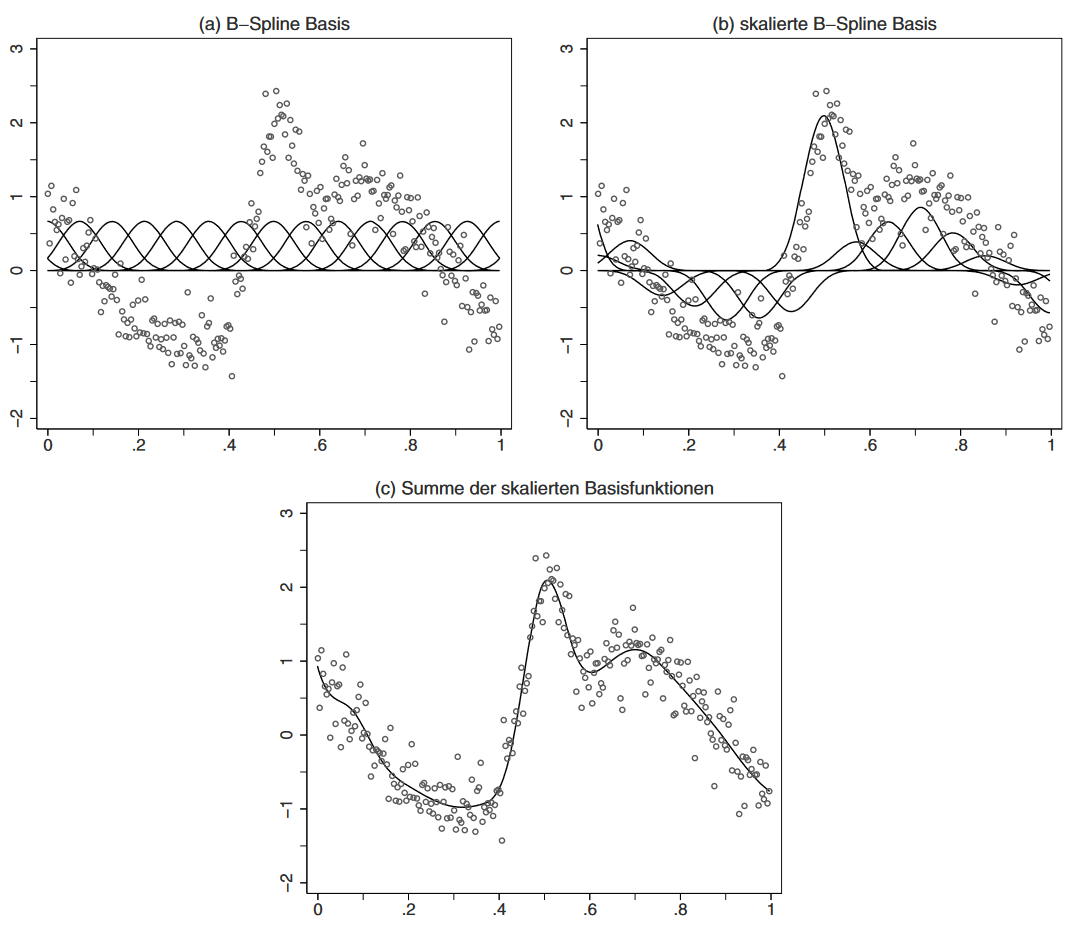
\includegraphics[width=.9\textwidth]{plots/b_spline.png}
	\caption{Schematische Darstellung der Schätzung eines nichtparametrischen Effekts mit B-Splines}
	\label{pic:b_spline}
\end{figure}

\noindent Das nächste Kapitel behandelt P-Splines, welche auf B-Splines basieren und durch einen Strafterm erweitert worden sind. In unserer Arbeit beschränken wir uns auf P-Splines.
\subsubsection{Penalisierte Splines basierend auf B-Splines}
	Im vorherigen Kapitel, haben wir die Wichtigkeit der Knotenmenge kennengelernt. Die Glattheit und Flexibilität der Schätzfunktion $f(z)$ hängt stark von der Anzahl der Knoten ab. Das Ziel ist es die Funktion $f(z)$ auf Basis einer B-Spline Funktion, mit einer großen Zahl an Knoten, zu approximieren um so die Flexibilität der Schätzfunktion sicherzustellen und andererseits zu hohe Variabilität in Form eines Strafterms zu sanktionieren. Der Penalisierte-Spline, gekürzt P-Spline, kombiniert somit eine B-Spline-Basis mit einem Strafterm. Der Strafterm für B-Splines wird häufig durch die quadrierte zweite Ableitung der Schätzfunktion $f(z)$ modelliert, da diese Form im R-Paket $mgcv$ von Simon Woods implementiert wird. Die zweite Ableitung stellt ein Maß für die Krümmung der Funktion dar und ist daher in der Lage die Glattheit einer Funktion einzuschätzen.
Der Strafterm: 
\begin{align}
\lambda\int(f''(z))^2dz.
\end{align}
In der Anwendung wird für die Approximation der zweiten Ableitungen, die zweite Differenz des Paramters $\gamma_{j}$ verwendet. Wenn der Glättungsparameter $\lambda$ gegen unendlich konvergiert, erhält man eine nahezu lineare Schätzfunktion $f(z)$ und der Strafterm wird primär durch $\lambda$ reguliert. Im Fall von $\lambda \to 0$ verfügt der Glättungsparameter ($\lambda$) nur über ein geringers Gewicht.
\subsubsection{Zyklische P-Splines}
Eine Glättungsfunktion hei"st $zyklisch$, wenn die Funktion dieselben Werte und ersten Ableitungen an ihrer oberen und unteren Grenze aufweist. Beispielsweise kann man die Funktion für die Variable Woche mit Hilfe von zyklische P-Splines modellieren. So könnte man sicher stellen, dass die Werte am Ende einer Woche zusammenhängend zu den Werten am Anfang der Woche sind. Beispielsweise könnte der Fall eintreten, dass Werte von Sonntag den Wert von Montag beeinflussen und andersherum. Der Penalisierungsansatz für zyklische P-Splines ist simultan zu der Penalisierung von P-Splines basierend auf B-Splines (siehe 4.6) \\

(\textbf{Simon Woods Buch in Bib leihen und Zyklische Splines weiter ausführen})



\end{document}


